\documentclass[12pt,a4paper]{article}
\usepackage[utf8]{inputenc}
\usepackage{amsmath}
\usepackage{amsfonts}
\usepackage{amssymb}
\usepackage{lipsum}
\usepackage{textcomp}

\usepackage{makecell} % linebreak dans une cellule
\usepackage{multicol} % twocols localement
\usepackage{vwcol} % idem mais avec largeur variable
\usepackage{color, colortbl} % colorer les tableaux
\usepackage{enumitem} % utiliser des lettres pour énumérer
\usepackage{wrapfig} % insérer des images dans dutexte
\usepackage{dashundergaps} % transformer du texte en ________
\usepackage{MnSymbol,wasysym} % smileys
\usepackage{minibox} % multiline fbox - \minibox[frame]{}
\usepackage[pscoord]{eso-pic} % floating text box \placetextbox{x}{y}{text}
\usepackage{ifthen}
\usepackage{soul} % teste barré \st

% --- geometry ---
\usepackage{geometry}
\geometry{legalpaper, margin=1cm}
% ---

% --- xcolor ---
\usepackage{xcolor}
\definecolor{lightgray}{gray}{0.9}
% ---

% --- tcolorboxes ---
\usepackage[most]{tcolorbox}
\newtcolorbox{definition}[2][]{%
  attach boxed title to top left
               = {yshift=-8pt},
  colback      = white,
  colframe     = gray,
  fonttitle    = \bfseries,
  colbacktitle = gray,
  title        = #2,#1,
  enhanced,
}
% ---

% --- array ---
\usepackage{array}
\newcolumntype{L}[1]{>{\raggedright\let\newline\\\arraybackslash\hspace{0pt}}m{#1}}
\newcolumntype{C}[1]{>{\centering\let\newline\\\arraybackslash\hspace{0pt}}m{#1}}
\newcolumntype{R}[1]{>{\raggedleft\let\newline\\\arraybackslash\hspace{0pt}}m{#1}}
 % ---


\renewcommand{\baselinestretch}{1.15} % augmenter l'interligne

\dashundergapssetup{
	teacher-gap-format=underline,
	gap-widen
}

\newcommand{\placetextbox}[3]{% \placetextbox{<horizontal pos>}{<vertical pos>}{<stuff>}
  \setbox0=\hbox{#3}% Put <stuff> in a box
  \AddToShipoutPictureFG*{% Add <stuff> to current page foreground
    \put(\LenToUnit{#1\paperwidth},\LenToUnit{#2\paperheight}){\vtop{{\null}\makebox[0pt][c]{#3}}}%
  }%
}%


\author{Paul Clavier}
\title{Chapitre 6 - Addition, soustraction, multiplication de nombres décimaux - Interrogation} 

\begin{document}

% --- Section & subsection renum ---
\renewcommand\thesection{\Roman{section}}
\renewcommand\thesubsection{\arabic{subsection}}
% ---

% --- Selection manuelle de la version ---
%\def\isprof{true}
% ---

% --- Selection automatique de la version ---
\ifdefined\isprof
	\TeacherModeOn
\fi

% ---

\begin{center}
	\minibox[frame,c]{Devoir surveillé 1}
\end{center}

\placetextbox{0.05}{0.99}{Nom:}
\placetextbox{0.05}{0.96}{Prénom:}

\begin{center}
\begin{tabular}{|l|c|}
\hline \rowcolor{lightgray}
Les nombres décimaux et géométrie \hspace{6cm} & Maitrise \\ \hline
\thead[l]{D1.3:1.2: Calculer avec des nombres entiers et des nombres  décimaux de manière \\ exacte ou approchée} &
\\ \hline
\thead[l]{D1.3:2.1: Utiliser des notions de géométrie plane} &
 \\ \hline
\end{tabular}
\end{center}

\textbf{Exercice 1}: Vocabulaire
3,6 × 4,5 = 16,2 \\

Complète les phrases qui suivent avec le vocabulaire adapté : \\

16,2 est \gap*{le produit} des nombres 3,6 et 4,5.\hspace{1cm} 3,6 et 4,5 sont les \gap*{facteurs} de la multiplication. \\

\begin{tabular}{|c|c|c|}
\hline
\thead{ 
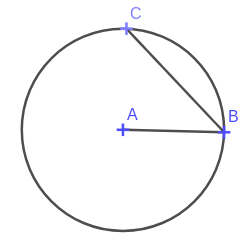
\includegraphics[scale=0.95]{img/DS-Cercle.png}\\
$[AB]$ est \gap*{un rayon} du cercle.\\
$[BC]$ est \gap*{une corde} du cercle.}
&
\thead{
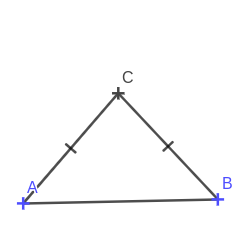
\includegraphics[scale=0.95]{img/DS-Triangle.png}\\
ABC est \gap*{un triangle isocèle}\\ \gap*{ de sommet principal C}}
&
\thead{
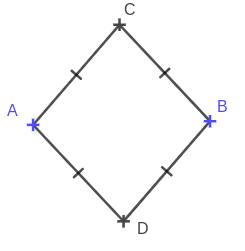
\includegraphics[scale=0.95]{img/DS-Losange.png}\\
ACBD est \gap*{un losange}\\
$[AB]$ est \gap*{un diagonale} 
 }
\\
\hline
\end{tabular}\\

\textbf{Exercice 2}: Pose et effectue les opérations suivantes

\begin{tabular}{|c|c|}
\hline 
\thead{17,04 + 8,7 \hspace{6cm} \vspace{5cm}} & \thead{21,17 - 6,2 \hspace{6cm} \vspace{5cm}} \\ 
\hline 
\thead{12,74$\times$3,8 \hspace{6cm} \vspace{8cm}} & 
\thead{4h26min + 2h43min \hspace{6cm} \vspace{8cm}}
\\
\hline 
\end{tabular}\\

\textbf{Exercice 3}: Calcul en ligne

\begin{tabular}{cc}
$2 543\times 0,01 =$ \gap*{25,43} & $34,7\times 100 =$ \gap*{3 470} \\ 
$0,14\times 1000 =$ \gap*{1 400} & $0,14\times 0,01 =$ \gap*{0,0014} \\ 
\end{tabular}\\

\newpage
\textbf{Exercice 4}: Suis le programme de construction en utilisant les points donnés

\begin{enumerate}
\item Trace le triangle équilatéral ABC de côté [AB] (conseil, place le point C au dessus du segment [AB])
\item Place D, le milieu de [BC]
\item Trace le triangle isocèle BCE, de base [BC] et de côté de longueur AD
\item Construit le rectangle CEFG, de largeur CE et de longueur AC
\end{enumerate}

\ifdefined\isprof
	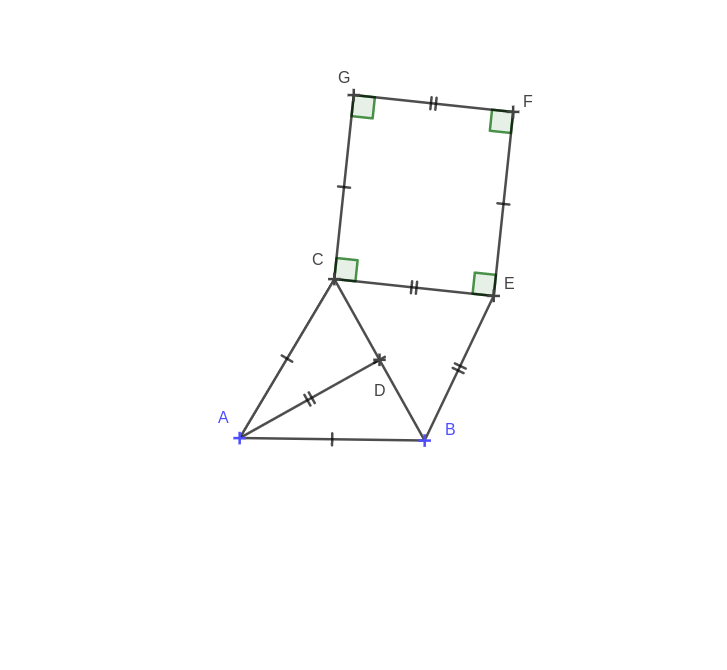
\includegraphics[scale=1]{img/DS-c.png} 
\else
	
\includegraphics[scale=1]{img/DS-s.png} 
\fi




\end{document}